\subsubsection*{The Problem}

The Wikipedia's continued success depends on ill-intentioned users
not being able to overwhelm the well-intentioned users.
Communities are complicated systems, with people constantly joining and
leaving membership.
We can suppose that people continue to
join the Wikipedia community because most pages are
substantially useful and users feel that their contributions
\textit{add} to the resource,
giving them a sense of satisfaction~\cite{Benkler2002}.
If the amount of vandalism occurring were to increase so that
most users were only \textit{repairing} the Wikipedia, there
would be much less satisfaction and eventually people would
leave the community --- a digital age tragedy of the commons~\cite{Hardin1968}.

\begin{figure}[t]
\centering
\subfigure[Before the modification~\cite{wiki:Denmark-Fogh}.]{
\label{fig-denmark-a} 
\framebox{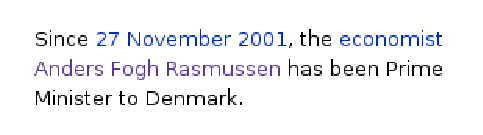
\includegraphics[width=0.45\textwidth]{part-C10-intro/Denmark-Fogh}}
}
\hspace{1ex}
\subfigure[Immediately after the modification~\cite{wiki:Denmark-Fjogh}.]{
\label{fig-denmark-b}
\framebox{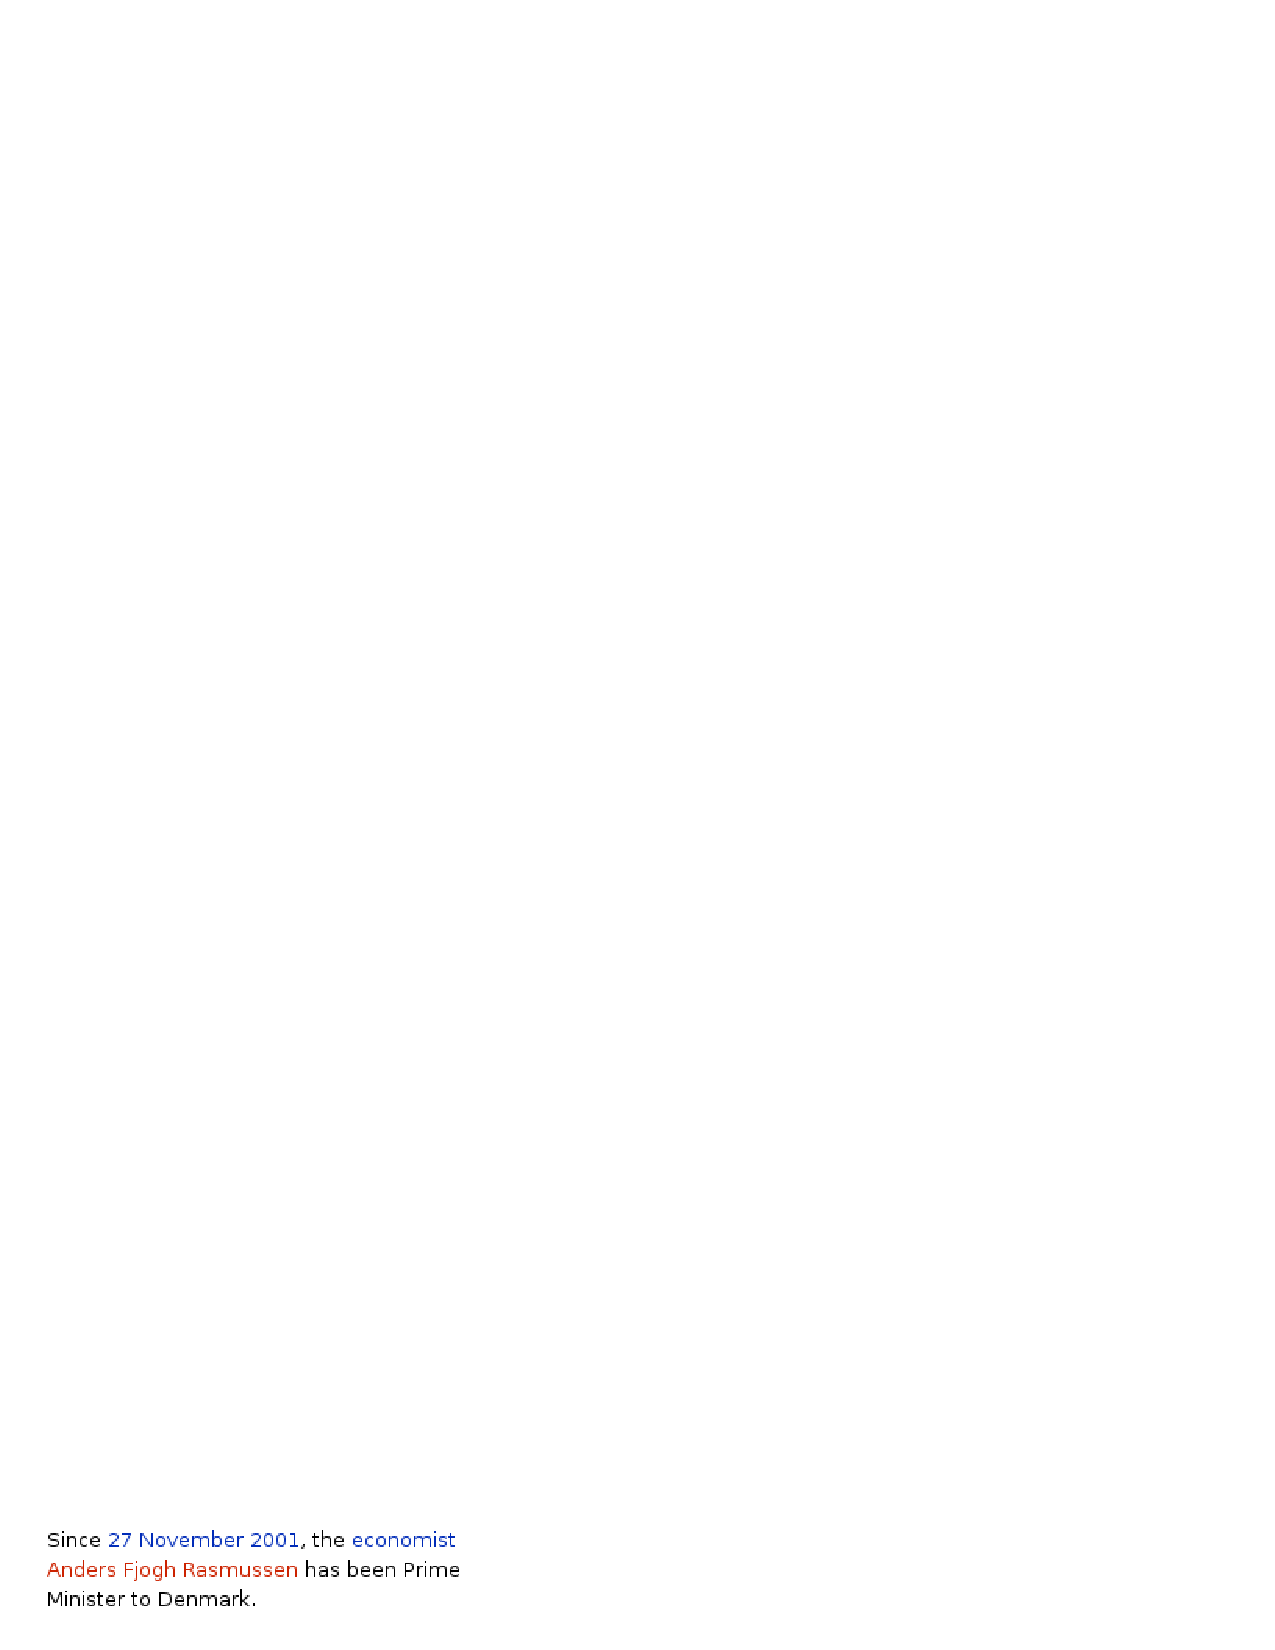
\includegraphics[width=0.45\textwidth]{part-C10-intro/Denmark-Fjogh}}
}
\caption{An attempt to modify the
  spelling of the Danish Prime Minister's last name, from Fogh, to Fjogh.
  The casual user who does not speak Danish, and happens to check
  the version history, has little indication on which might be correct.
  In fact, this is a case of vandalism
  (in Danish, a \textit{fjog} is a \textit{fool})
  that is quite subtle and wouldn't even be noticed by most users.}
\label{fig-denmark}
\end{figure}


Vandalism can be very hard to identify for inexperienced users.
Consider the example of Figure~\ref{fig-denmark},
which is an excerpt from the ``Politics of Denmark''
entry in the English Wikipedia: an anonymous user substitutes
``Fjogh'' for ``Fogh'' in the Prime Minister's last name.
This is a particularly subtle kind of vandalism,
because it requires knowledge of Danish
(\textit{fjog} translates to \textit{fool} or \textit{goofy})
to recognize this change as anything more than a spelling correction.
A sophisticated reader might recognize the broken link
as a hint on the true spelling, or even try to use Google
to research the name (both spellings return results, however).
The level of effort to recognize the error and
verify this relatively small detail is quite high.

